% \lecture{4}{Tue 04 Feb 2020 14:30}{393 Lab 4}

\section{Plots of System response varying $\omega_{0}$, $\zeta$}
The result of varying $\zeta$ is the graph in Figure \ref{fig:varying-zeta}.
\begin{figure}[H]
	\centering
	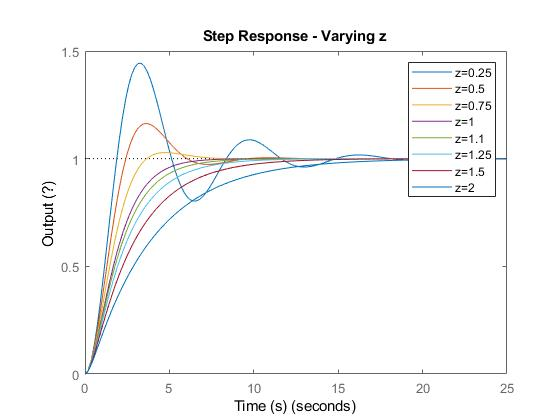
\includegraphics[width=0.8\textwidth]{./figures/lab4_fig1-part4-3-1-z.jpg}
	\caption{A plot of the system response when varying the value of $\zeta$}
	\label{fig:varying-zeta}
\end{figure}
As you can see an increase in $\zeta$ increases the damping of the output, where $\zeta=1$ seems to be close to the critical damping value, $\zeta < 1$ is an underdamped system and $\zeta > 1$ is an overdamped system. 

The result of varying $\omega_{0}$ is seen in Figure \ref{fig:varying-w0}.
\begin{figure}[H]
	\centering
	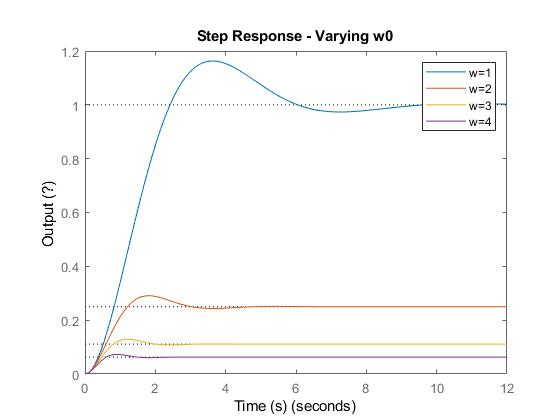
\includegraphics[width=0.8\textwidth]{./figures/lab4_fig2-part4-3-1-w0.jpg}
	\caption{A plot of the system response when varying the value of $\omega _{0}$}
	\label{fig:varying-w0}
\end{figure}
The greater the value of $\omega_{0}$, the smaller the steady-state value of the system. 

\section{Effects of Changing $\alpha$}  %Maxym
For positive values of $\alpha$, the effect of increasing $\alpha$ is the graph in Figure \ref{fig:varying-alpha-positive}.
\begin{figure}[H]
	\centering
	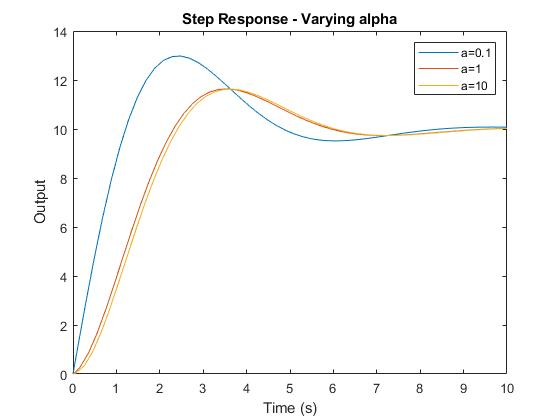
\includegraphics[width=0.8\textwidth]{./figures/lab4_fig3-part4-3-2-positive.jpg}
	\caption{A plot of the system response when varying the positive values of $\alpha$}
	\label{fig:varying-alpha-positive}
\end{figure}
As $\alpha$ increases, the rise time of the system also increases. While there is a large difference between the rise times of $\alpha = 0.1$ and $\alpha = 1$, the difference between $\alpha = 1$ and $\alpha = 10$ is relatively small. Meanwhile, settling time for all positive values of $\alpha$ appear relatively similar with all of the values converging to 10 at approximately 10 seconds. All three positive values of $\alpha$ displayed overshoot with $\alpha = 0.1$ having the largest overshoot while $\alpha =1$ and $\alpha = 10$ had smaller overshoots. Similarly, the peak time of $\alpha = 0.1$ is much shorter than the peak times of $\alpha = 1$ and $\alpha = 10$. The graph shows that $\alpha = 10$ has the longest peak time. 

For negative values of $\alpha$, the effect of increasing $\alpha$ is the graph in Figure \ref{fig:varying-alpha-negative}.
\begin{figure}[H]
	\centering
	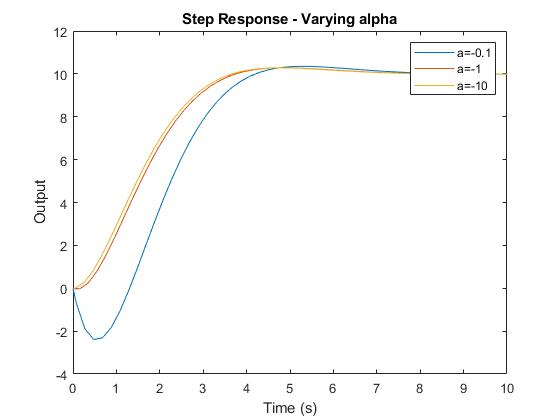
\includegraphics[width=0.8\textwidth]{./figures/lab4_fig4-part4-3-2-negative.jpg}
	\caption{A plot of the system response when varying the negative value of $\alpha$}
	\label{fig:varying-alpha-negative}
\end{figure}
As $\alpha$ increases negatively, the rise time of the system decreases. While there is a large difference between the rise times of $\alpha = -0.1$ and $\alpha = -1$, the difference between $\alpha = -1$ and $\alpha = -10$ is relatively small. Meanwhile, settling time for all negative values of $\alpha$ appear relatively similar with all of the values converging to 10 at just under 10 seconds. All three negative values of $\alpha$ displayed small overshoot with $\alpha = -0.1$ having a slightly larger overshoot than $\alpha =1$ and $\alpha = 10$. The peak time of $\alpha = -0.1$ is slightly longer than the peak times of $\alpha = 1$ and $\alpha = 10$ which had similar peak times.
% End Maxym Section

\section{Why Are The Plots The Same?}


\section{System Type Section}

% we can just toss the values in as a screenshot of the excel docs

steady state error for $R_{c} = 5$ : -0.021496
